\chapter{Human-Computer Interaction and User Centered Design}
\label{ch:hci}
\section{HCI and Human-Centred Design.}
The science of \gls{hci} studies the interaction between humans and computers. The goal is to make this interaction as smooth and seamless as possible. Research done in the \gls{hci}-field have resulted in guidelines and design methods for the creation of efficient and usable software. One important factor when focusing on usability is to include the future users the design process to get feedback on the user interface.

ISO 9241-210 provides guidance and acts as a usability standard for human-computer interaction throughout the life cycle of interactive systems. The ISO takes a human-centred design approach to interactive system development. According to the ISO the aim of human-centred design is to make systems usable and useful by focusing on the users, their needs and requirements, and by applying human factors and usability knowledge and techniques \cite{iso9241}.

\begin{figure}[h!]
	\centering
		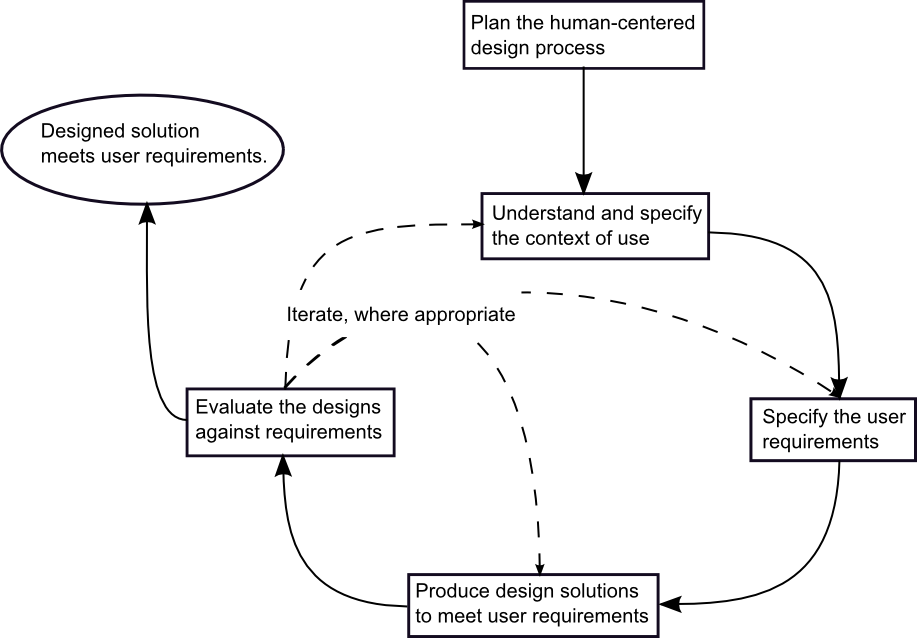
\includegraphics[width=0.9\textwidth]{hcdActivities.png}
		\caption{\footnotesize The human-centred design workflow}
		\label{fig:hcdActivities}
\end{figure}

The standard describes 6 key principles, as listed below. These principals in combination with figure~\ref{fig:hcdActivities} will ensure that the design is user centred. The figure is in no way a strict linear process to follow, it merely shows the required input and expected result of each activity.

\begin{enumerate}
  \item Users are involved throughout design and development.
  \item The design team consists of members with varied backgrounds
  \item The design is based upon an understanding of users, tasks and environments.
  \item The design is driven and refined by user centred evaluation.
  \item The process iterative.
  \item The design addresses the whole user experience.
\end{enumerate}

The first principle emphasizes user involvement throughout the entire process, and not just at the start and the end of the system design, but through the entire cycle of activities. It is important to include a wide range of views and input from experts in various fields, this is where the second principle comes in. It ensures that not everyone thinks and approaches the problem in the same way. The third principle involves understanding the user, what they want to do with the system, and the environment the system will be used in, this is sometimes referred to as the \textit{user experience trinity}. 

Principle 4 and 5 address the fact that several iterations might be required for a satisfactory design to be reached. Users might not know what they want, but they do know what they do not want once they have experienced it. Multiple iterations and examples may then be required to find something that is satisfactory to the user. The final principle states that the usability is not just about making things easy to use, but provide the user with a emotional and perceptive stimuli as well. They should wish to use the system and feel good about it.

\section{Information Visualization}
%DENNE SEKSJONEN TRENGER FLERE BILDER FOR � ILLUSTRERE POENGET V�RT.SJEKK https://www.interaction-design.org/ UNDER DATA DOCUMENTS, VI KAN OGS� BRUKE BILDER FRA D3JS.
Information visualization is useful when you want to display large amounts of data simultaneously. The human brain is not good at getting an overview of the information by looking at large tables of numbers or text. Visualizations utilize the strengths of human cognition. By using computer graphics to make visualizations, large amounts of information can be displayed in a way that humans can process and analyse quickly and intuitively.

Many guidelines have been suggested for creation of the optimal visualization. Shneiderman summarized many of these principles in his \emph{visual-information-seeking mantra}~\cite{shneiderman}:

\vspace{-13pt}
\begin{quote}
\textit{Overview first, zoom and filter, then details on demand.}
\end{quote}

For the visualization to be effective the user has to get an overview of how the information is presented. The system should also allow for zooming in on interesting parts of the information as well as giving the opportunity to filter out information that is not of interest. Most visualizations remove some level of detail for the data to be more accessible and easier to read. Therefore it is important that the system allows the user to access more detailed data when needed.

Shneiderman also identifies the importance of showing the relationships between different items, allowing the user to extract subcollections of the displayed items and storing the user action history to allow for undo/redo functionality.

\subsection{Visual Variables} 
// This section needs descriptive illustrations, see www.interactin-design.org (article at the bottom).

One important factor to consider when creating a visualizations are which visual variables to use. To create an intuitive visualization it is important use the different visual variables correctly. We will briefly go through some of the more common visual variables here and discuss how and how not to use them, based on Carpendales article about the subject~\cite{carpendale}.

\textbf{Visual variables:}
\begin{table}[h!]
  \begin{tabular}{|l|p{10cm}|}
      \hline
      Position    & Position of object, for example x- and y-coordinates in a two dimensional system. \\ \hline
      Size        & Size of object. \\ \hline
      Value       & Change in colour scale from light to dark. \\ \hline
      Colour      & Change hue for given value, for example blue, red and yellow. \\ \hline
  \end{tabular}
  \caption{Overview of visual variables.}
\end{table}

\textbf{Characteristics of visual variables:}
\begin{table}[h!]
  \begin{tabular}{|l|p{10cm}|}
      \hline
      Selective   & Will a change in this variable make it easier to select it from a group of variables? \\ \hline
        Associative & Will changes in variables make us able to distinguish different groups of variables \\ \hline 
        Qualitative & Can the visual variable be used to illustrate the numerical value and relationship between variables? \\ \hline
        Order       & Will changes in the visual variable allow us to order them? \\ \hline
        Length      & How many changes is it possible to distinguish between for this type of variable? \\ \hline
    \end{tabular}
    \caption{Description of characteristics of visual variables}
\end{table}

Position fulfils all the characteristics of visual variables. When thinking of a scatter plot it is easy to see that positioning the points will make them selective and associative. By using scales, position can be used to show the value of the variable in a numerical sense, so it is also quantitative. Order is also fulfilled, a ruler is a simple example of how position can be used to order. The length is theoretically infinite, and only restricted by the screen resolution.

Size fulfils all of the characteristics. It is both selective and associative, humans can easily identify for example the smallest circle in a group of circles. Though size can be used to visualize a numerical value, it is often hard for humans to accurately see how much larger one object is compared to another. Different sizes can easily be ordered. As for the length of this variable Carpendale suggest about five different sizes for selection and about 20 different sizes for distinction. It is important to note that humans can identify small changes in size when objects are close, however when the distance between objects is increased it is hard to distinguish between these differences.

Value can be used both for selection and association. Humans can identify darker parts and group them with ease. It is not quantitative, it is difficult to identify that one tone of grey is twice as dark as another. One can however say that one grey tone is darker than another, and therefore you can order them. Carpendale suggest that the length of this variable is less than 7 for selection, and about 10 for distinction.

Colours are selective and associative. Unless you are colour blind you can easily identify and group different colours. Colours are not quantitative, it is hard for humans to say that one colours is twice that of another. Though we have colour scales, humans do not intuitively order colours, this can easily be illustrated by a question: Which colours is greater blue or yellow? Most people will not have an answer. Carpendale suggests that you use less than 7 different colours for selection, and about 10 for distinction.

\subsection{Interactivity}
One of the benefits of creating visualizations for computers is the ability to add interactivity. Shneidermann mentions 6 tasks that should be implemented when creating information visualizations:
\vspace{-3mm}
\begin{description}[itemsep=0cm, parsep=0cm]
  \item[Overview] Show an overview of the entire data set
  \item[Zoom] Let the user look closer at elements of interest
  \item[Filter] The user should be able to filter out tasks that are not interesting
  \item[Details-on-demand] Show details when elements are selected
  \item[History] Let the user undo or redo actions
  \item[Extract] Allow the user to extract a subset of the entire data set
\end{description}

The first thing the users sees when interacting with an information visualization is an overview of the data set. This can be done by zooming out and then let the user zoom in on areas of interest. Another approach is to aggregate the data in separate sections that can then be investigated further.

It is rare that the user is equally interested in every part of the data set, therefore it is useful to be able to zoom in on elements for a more detailed look. It is important to make sure that the user does not loose their sense of position and get lost in the visualization.

Often the some of the data in the set is not relevant and only distorts the visualization. In such cases one should be able to filter out those elements. The user should be able to filter out unwanted data using sliders, buttons etc. The update should happen real-time, to allow the user to see how the filter affects the visualization. 

Typically information visualizations hide the numerical data (or other detailed data) behind the element. It is therefore paramount to give the user the ability to access this data when it is needed. The user should be able to select an element or a small group of elements and browse the details in a list or other textual representation.

When working with a visualizations where you can make changes to filter, zoom, etc. It is useful for the user to be able to undo and redo tasks. Undo will give the user the ability to go back form an undesired zoom level or filter setting quickly. Users will often times do make more actions than they can keep track of, so giving them the ability to trace their steps improves usability.

When the user has used the visualization and found what he was looking for, the user should be able to extract those elements. The extracted elements should be saved in a format that can be sent to and seen by others. 

\section{Interview}
By performing an interview the interviewer wishes to acquire knowledge from the subject (interviewee) through a conversation. Interviews can be unstructured, semi-structured or structured~\cite{interactionDesign}.
\begin{description}
  \item[Unstructured interviews] are exploratory conversations around a certain topic or area of concern. These can be completely informally.
  \item[Semi-structured interviews] follow a general guideline or script that serve as a checklist and provide consistency between interviews. The order and wording can be freely modified to follow the conversation flow, and unplanned follow up questions are often asked.
  \item[Structured interviews] have set of predefined questions with fixed wording and are in a pre-set order. It is much like a questionnaire but allows for slightly more open-response questions.
\end{description}
Ideal structure choice for an interview is decided by its purpose, what questions need to be addressed and how far has development come? If the goal is to gain first impressions, initial design ideas or information about a particular topic then unstructured interviews are often the best approach. A more structured approach is useful when the goal is to get feedback on particular design features such as the layout of a website, in such cases  structured interviews or semi-structured interviews are useful.

% REVIEW: You can mention that interviews are less prone to have problems with the subjects not understanding the question, because the interviewer can explain the questions and what was meant.
The advantage with interviews is that they are flexible and easy to alter prior or during an interview session. The interviewer gets an immediate response from the subject, and can change accordingly if the interview is not working as planned. Interviews do have drawbacks, conducting and transcribing interviews are both time a time consuming process. Bias might also be presents where the subject being interviewed says things he believes the interviewer wants to be hear or neglects to provide information. This might particularly be the case when the interview has gone on for too long and the participant wants it to end \cite{realWorldResearch}.

\section{Brainstorming}
Brainstorming is a generic technique used to generate, develop and refine ideas. It is widely used in interactive design to generate alternative designs and provide better ideas for certain problems~\cite{interactionDesign}. The technique has no real structure or rules, but in addition to the list below the book, \textit{Interaction Design: Beyond Human-Computer Interaction}, mentions two key success factors: Participants should know the user goals that the system is intended to support, and that no ideas should be criticized or debated, everything is initially accepted.

\begin{enumerate}
  \item Participants should ideally be from a wide range of disciplines and have a broad range of experience.
  \item Do not exclude unconventional ideas, these can often be turned into useful requirements.
  \item Build one idea on top of another. Suggest jumping back to an earlier an idea if the vigour diminishes. Use a random word from the dictionary and related it to the product if stuck.
  \item Keep records without censoring, and number them so jumping back to previous ideas is easy. Participants should be encoraged to sketch, create diagrams, and keep notes.
  \item Staying focused is important. Having a well articulated and honed problem helps focus people and direct the session back on topic if it wanders.
  \item If the participants are unfamiliar with each other it is important to have warm up exercises such as word games or exploring physical objects available to them.
\end{enumerate}

\section{Prototyping}
A prototype is a realization of a design that stakeholders can interact with and explore. The limitation of a prototype is that it often only focuses on one product characteristic and neglects the others. A prototype can be anything from a complex piece of software to a simple storyboard or sketch. Prototypes serve as an aid by clarifying communication between team members, and efficiently exploring design ideas with stakeholders and designers. Building the prototype itself encourages reflection of the design and is recognized by designers from many disciplines as an important aspect of the design process \cite{interactionDesign}.

\subsection{Low-fidelity vs. High fidelity}
Low-fidelty prototypes do not resemble the finish product very much. It often uses completely different and much cheaper materials then the final product making them cheap, simple and easily modifiable. Examples of such prototypes are storyboards, sketching, and wizard of Oz. Low-fidelity are important in early development stages because the simplicity encourages exploration and modification. The disadvantage is that these prototypes are never kept or integrated into the final product.

High-fidelity prototypes are much closer to the final product, and therefore give a much stronger impression of the final product. The high-fidelity prototype is useful for identifying technical issues and selling ideas to people. These prototypes are often reused or developed into a final product, but require more time and resources to create.

The very nature of a prototype involves making compromises. Therefore the choice of prototype lies in what kind of of questions we want to answer. Two common compromises that are often traded against each other are breadth of functionality vs depth of functionality. \textit{Horizontal prototyping} focuses on a wide range of functions but little details and \textit{vertical prototyping} focuses on providing a lot of detail for a few functions. 

\subsection{What do prototypes prototype?}
In the article \textit{What do Prototypes Prototype}~\cite{prototypesPrototype} Houde and Hill discuss how prototypes need to be designed to test or rather prototype a certain design aspect of the final product. The model shown in Figure~\ref{fig:hillTriangle} represents a three dimensional space which corresponds to important design aspects of an interactive system. Each corner of the triangle represents a set of questions which are essential to the design of a system. \textit{Look and feel} covers questions that concern itself on what the user feels, sees and hears when using the system, in other words the sensory experience. \textit{Role} as the name states refers to questions about what role the system has in the users life, what function does it server and how is it useful to them. \textit{Implementation} addressed the technical aspects of the system, what techniques and components are should be used for it to be able to perform the intended function. The triangle is intentionally skewed to emphasize that no set of questions is more important than the other.
%WRITE ABOUT HOUD AND HILLS TRIANGLE OF AWESOMNESS http://hci.stanford.edu/courses/cs247/2012/readings/WhatDoPrototypesPrototype.pdf

\begin{figure}[h!]
	\centering
		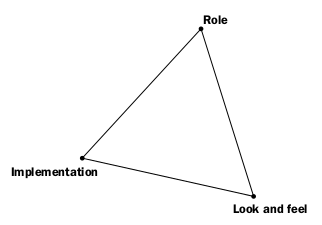
\includegraphics[width=0.6\textwidth]{hillTriangle.png}
		\caption{\footnotesize The prototype triangle by Houde and Hill~\cite{prototypesPrototype}}
		\label{fig:hillTriangle}
\end{figure}

The purpose of the model is to help designers seperate design issues into the three aforementioned set of questions, which often require very different approaches to prototyping. Look and feel requires the user experience to be created or simulated, implementation requires a running system to be built, and role involves researching the use context for the system. Categorizing the important design questions will help decide on what kind of prototype should be built and focus the exploration.

\section{Focus groups}
Focus group, or group interview is an informal technique that can help software developers identify the users needs and feelings about a system. The technique can be used both before interface design and long after the system has been implemented. 

According to Nielsen~\cite{focusGroup} the focus group should have at least six participant to maintain a flowing discussion and provide different perspectives. The participants should be representative of the intended users, or be the final users themselves. Sessions normally last two hours and are run by a moderator. The moderators job is to keep the discussion flowing and let everyone get their point across. Moderators can also guide the discussion in the direction relevant to the goals of the focus groups. 

A single session may not be representative enough or can get sidetracked, it is therefore important to run more than one focus group. If improvements suggested by participants have been implemented it is important to run another iteration of the focus group with the same participants to attain feedback on the changes that have been made. Enough focus groups have been conducted when new information is no longer being received, i.e. a point of saturation has been reached~\cite{howFocusGroup}. 

Nielsen~\cite{focusGroup} discusses two pitfalls with focus groups: Because sessions are in groups the users do not test the system themselves, instead they are presented with a demo. The problem with such a demo is that the participants never have to question what to do next or consider the meaning of the screen options. The second problem is that what participants say they want, is not necessarily what they need. Also, ideas described by the moderator might be perceived differently by the participants. By providing concrete examples through prototypes of the technology, one can minimize this problem.

\section{Questionnaire}
Questionnaires are a research tool that consist of a series of questions with the goal to attain information from the respondent. It is a well established technique for collecting demographic data and user opinion, they are similar to an interview in the fact that they can contain both closed and open ended questions. Clear unambiguous questions and allowing efficient data collection is important, especially if a large quantity of questionnaires have been issued. Questionnaires can be used on their own or as an addition to other methods in order to gain background information, or deepen understanding of a particular topic. Below is a short and general guideline provided by~\cite{interactionDesign} on things to watch our for when creating questionnaires.

\begin{itemize}
  \item The order of which questions appear is important, it can influence the impact of a question.
  \item Consider having alternate versions of the questionnaire to suit different populations.
  \item Clear instructions on how the questionnaire should be filled in essential. Clear wording and good typography is important.
  \item Balance must be attained between whitespace and needing to keep the questionnaire as short as possible. Long questionnaires cost more, and might deter people from participating.
\end{itemize}

The advantage with questionnaires is that hey provide relatively simple and forward study, and may be adapted to collect generalized information from almost any human population which means high amounts of data standardization. If the survey is anonymous it can encourage more honesty then another research method would have if sensitive topics are involved. In addition to being relatively cheap to perform compared to the amount of data that is gathered. There are downsides this form of data collection, people might respond in a way that puts them in a good light, and data is affected by the respondents characteristics. Their memory, knowledge, experience and motivation influence how they answer the survey. A downside with questionnaires without any kind of monitoring are ambiguity or misunderstanding in the survey questions that is never detected, respondents might not take the questionnaire seriously, or there are low response rates.

\section{Validity}
According to \textit{Interaction Design: beyond human-computer interaction} validity is concerned with whether the evaluation method measures what it is intended to measure. This applies to both the method itself and the way it is executed. For example, if one wishes to examine how a product is used in the home, setting up a controlled lab experiment would hurt the validity. Wrong choice of method and execution are not the only threats to validity, bias and the Ecological Validity threaten the validity but can be impossible or hard to avoid.

Ecological Validity is concerned with how the evaluation method and environment themselves influence and affect the results. If a subject is aware of being observed and the test is conducted outside of their natural surroundings their behaviour and answers will be influenced. Bias is when the results are distorted by the researchers and evaluators. Evaluators might fail to note certain behaviour because they deem it irrelevant, or an interviewers tone of voice may influence the answers of the interviewee. It is therefore important to be open to the possibility of bias.

Validity in \gls{hci} is a complex area and we have only mentioned some of the basic issues. Thimbleby reviews some of the more complex issues and suggests some practical recommendations for solving them in his \textit{Validity and Cross-Validity in HCI Publications} paper \cite{validation}. One of the simpler suggestion he makes is to use Triangulation. Triangulation involves using multiple methods or sources to achieve the same result. A more elaborate method to assure good validity involves creating a universal star rating system, where papers should be rated based on how easily a researcher can reproduce or build upon the original work.

